This annex is dedicated to the explanation of details of the Japanese language that are relevant to the context of this work.

\section{Romanization}\label{ape:romanization}
The concept of romanization is the application of Latin letters to transcribe the Japanese language. This form of writing is sometimes referred as r\={o}maji (\jap{ローマ字}, literally "roman letter"). There are a number of different romanization methods, but one of them is by far the most widely used: the Revised Hepburn romanization. This system generally follows English phonology to transcribe Japanese in a way that is intuitive to English speakers. Most of the English versions of cities names are derived from slight modifications of this method. Table \ref{hepburntab}.

\begin{table}[h]
\centering
\caption{Comparison of city names to its Hepbrun Romanizations}
\label{hepburntab}
\begin{tabular}{|c|c|c|}
\hline
\textbf{Hiragana} & \textbf{Hepburn Romanization} & \textbf{English Name} \\ \hline
\jap{おおさか}        & \={O}saka                     & Osaka                 \\ \hline
\jap{とうきょう}       & T\={o}ky\={o}                   & Tokyo                 \\ \hline
\jap{なごや}         & Nagoya                        & Nagoya                \\ \hline
\end{tabular}
\end{table}


\section{Hiragana and Katakana}\label{hirakata}
Hiragana and Katakana are syllabic components of the Japanese writing system, and are referred as Kana scripts. Those two alphabets serve to fulfill syntactical roles in Japanese, as well as to spell some words and as a sort of subtitle of Kanji characters considered to be difficult to read by the reader. Most substantives, root of verbs, adjectives and adverbs are written in Kanji, while the conjugations of these verbs, adjectives and adverbs, indicative particles and some few words are written solely in some Kana script.

Hiragana is the most commonly used script, while Katakana is used on in special cases, such as describing a word alien to Japanese (a borrow word) or to give textual emphasis. Having two forms to write the same grapheme is already something common in the Latin alphabet, which is a Bicameral script\footnote{A type of script that have two forms for every grapheme, one that is said to be the lower case and the other said to be the upper case.}, but in Japanese this second script is not intermixed within the same word. One analogy that could be made to our writing system would be writing words to be emphasised at all caps. To clarify this concept, let us look at an example.

\begin{center}
\jap{{\Large ネコ} が {\Large ライス} を食べている}\\
NEKO ga RAISU wo tabeteiru\\
the CAT is eating RICE.
\end{center}

In this example, the enlarged characters are in Katakana, while the rest is in Hiragana or Kanji. Although "Neko" (cat) is a Japanese word, it is written in Katakana here to give stress to this word. The second word in Katakana is "Raisu" which is an English borrow word for rice.

In modern Japanese, each of these scripts is formed by 46 unique graphemes, to be added to 25 additional variation graphemes\footnote{These variations are created through the addition of a voicing mark called the dakuten. For example, we have the pure letter \jap{は}(ha) that can also be voiced as \jap{ば}(ba) and \jap{ぱ}(pa).} and one consonant voicing mark, \jap{っ}, the small "tsu". Both these scripts are displayed in figure \ref{hirakata}.

\begin{figure}[ht]
    \centering
    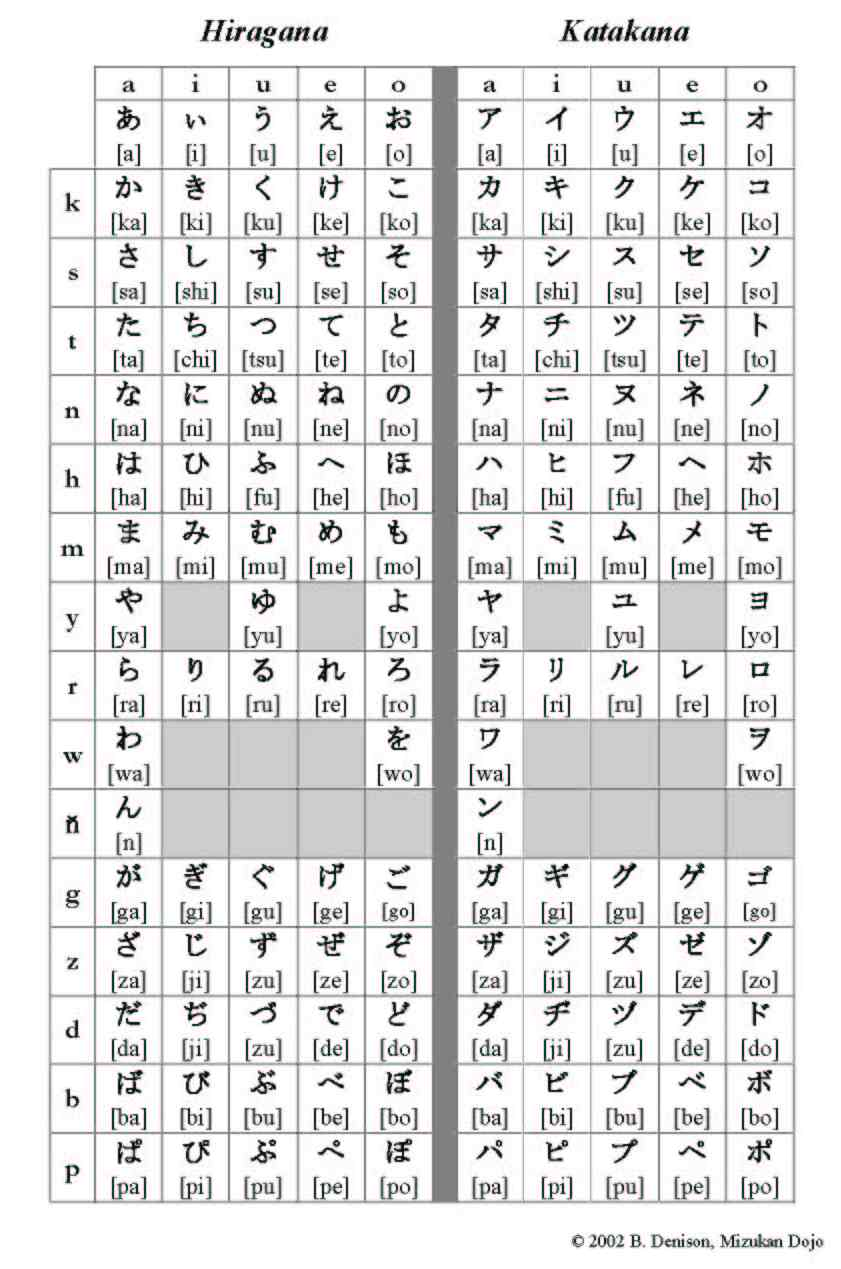
\includegraphics[width=0.9\textwidth]{ApeB/HiraKata}
    \caption{Hiragana and Katakana Scripts}
    \label{fig:hirakata}
\end{figure}